\chapter{Dataset Introduction} % Main chapter title

\label{Chapter 3} 
\lhead{Chapter 3. \emph{Dataset Introduction}} 

In this chapter, we will discuss the dataset and data analysis. 
Data set for Bharatanatyam Adavus is not open-sourced for research purpose.

\section{Dataset Introduction}
 So, We have recorded different dance formats for Adavus Bharatanatyam with the help of experts, dancers and learners. For the creation of dataset for Bharatanatyam adavus, Microsoft Kinect \cite{wiki:002} is used to capture RGB, skeleton videos and depth at a rate of 30 frames per second (fps).
 
\begin{figure}[hbt!]
  \centering
  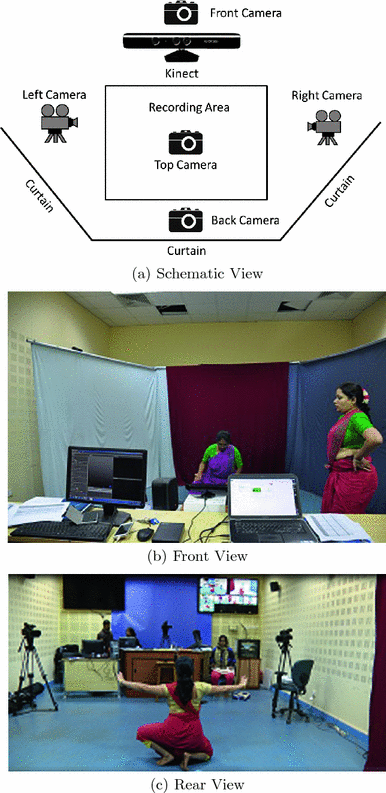
\includegraphics[scale= 0.5]{./Pictures/setup.png}
  \caption{Bharatanatyam Studio setup for recording}
  \label{fig:Ch03F001}
\end{figure}
The setup used for recording data set is shown in Figure \ref{fig:Ch03F001}

In this section of the project, only RGB frames are required for research purpose. Our approach was using a set of standard RGB as input and resized from 480 x 640 to 120 x 160 RGB frames, which had been further converted to grey frames for background subtraction.


The following Adavus had been recorded as a data set.
\begin{enumerate}
    \item Joining
    \item Kartari
    \item Nattal 
    \item Tattal 
    \item Mandi
    \item Mettu 
    \item Natta 
    \item Paikal
    \item Pakka
    \item Sarika 
    \item Sarikkal
    \item Tatta 
    \item Tei-Tei Dhatta
    \item Tirmana
    \item Utsanga
\end{enumerate}

\begin{table}[]
\hspace{-3cm}
\begin{tabular}{|c|c|c|c|c|c|c|}
\hline
\textbf{ADAVU} & \textbf{Variant} & \textbf{\# Dancers} & \textbf{\# Videos} & \textbf{\# Frames} & \textbf{\# Motion Frame} & \textbf{\# Key Frame} \\ \hline
\textbf{Tatta}          & 8  & 3 & 24  & 27155  & 12531 & 14624 \\ \hline
\textbf{Natta}          & 8  & 3 & 24  & 18587  & 9546  & 9041  \\ \hline
\textbf{Kuditta Mettu}  & 4  & 3 & 12  & 8895   & 4325  & 4570  \\ \hline
\textbf{Kuditta Nattal} & 6  & 3 & 18  & 15743  & 9816  & 5927  \\ \hline
\textbf{Kuditta Tattal} & 5  & 3 & 15  & 20995  & 13424 & 7571  \\ \hline
\textbf{Tei Tei Dhatta} & 3  & 3 & 9   & 5598   & 4336  & 1262  \\ \hline
\textbf{Katti Kartari}  & 1  & 3 & 3   & 2449   & 1747  & 702   \\ \hline
\textbf{Utsanga}        & 1  & 3 & 3   & 1363   & 1085  & 278   \\ \hline
\textbf{Mandi}          & 2  & 3 & 6   & 9975   & 5449  & 4526  \\ \hline
\textbf{Tirmana}        & 3  & 3 & 9   & 6415   & 4181  & 2234  \\ \hline
\textbf{Sarika}         & 4  & 3 & 12  & 8492   & 5662  & 2830  \\ \hline
\textbf{Joining}        & 3  & 2 & 6   & 4460   & 3110  & 1350  \\ \hline
\textbf{Total}          & 48 &   & 141 & 130127 & 75212 & 54915 \\ \hline
\end{tabular}
\caption{Bharatanatyam, Data set introduction}
\label{tab:Ch01T01}
\end{table}

Each Adavus have different numbers of variants. For each variation, three different dancers have performed Bharatanatyam dance. The data set has been shown in Table \ref{tab:Ch01T01}

After analyzing the dataset, we have observed that the annotation file for some of the Adavus and variation are not available. So, we have removed it from here as it is not relevant for us.

\begin{figure}[hbt!]
\centering
  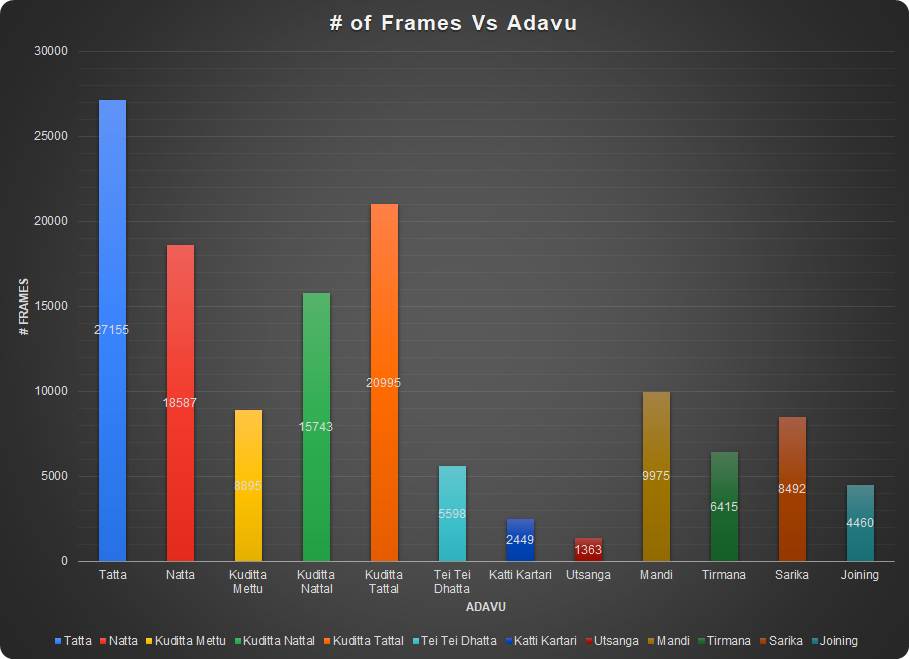
\includegraphics[scale= 0.8]{./Pictures/DataSet_Introduction.png}
  \caption{Bharatanatyam,Pictorial representation Data set}
  \label{fig:Ch03F002}
\end{figure}


\begin{table}[]
\centering
\begin{tabular}{|c|c|c|}
\hline
\textbf{ID}         & \textbf{Start Frame \#} & \textbf{End Frame \#} \\ \hline
\textbf{D1T4P01B1}  & 267                    & 303                  \\ \hline
\textbf{D1T4P01B2}  & 315                    & 350                  \\ \hline
\textbf{D1T4P01B3}  & 361                    & 396                  \\ \hline
\textbf{D1T4P01B4}  & 409                    & 444                  \\ \hline
\textbf{D1T4P01B5}  & 458                    & 494                  \\ \hline
\textbf{D1T4P01B6}  & 507                    & 542                  \\ \hline
\textbf{D1T4P01B7}  & 554                    & 590                  \\ \hline
\textbf{D1T4P01B8}  & 603                    & 643                  \\ \hline
\textbf{D1T4P01B9}  & 656                    & 684                  \\ \hline
\textbf{D1T4P01B10} & 697                    & 728                  \\ \hline
\textbf{D1T4P01B11} & 742                    & 775                  \\ \hline
\textbf{D1T4P01B12} & 788                    & 821                  \\ \hline
\textbf{D1T4P01B13} & 834                    & 865                  \\ \hline
\textbf{D1T4P01B14} & 879                    & 912                  \\ \hline
\textbf{D1T4P01B15} & 924                    & 953                  \\ \hline
\textbf{D1T4P01B16} & 966                    & 996                  \\ \hline
\end{tabular}
\caption{Tatta, Variant 4, Dancer 1 annotation file}
\label{tab:Ch01T02}
\end{table}


Each Adavu follows a regular pattern; for two consecutive Keyframe, there exist motion frames. All frames before 267, i.e., 1 to 265, are dancer preparing frame so that we would discard all frames. For example, in the first row, 267 is starting a Keyframe, and 303 is ending the Keyframe. After 303, i.e., from 304 to 314 are motion frames, and again Keyframe would be repeated similarly in Table.\ref{tab:Ch01T02}
